% Insert result section here. 
\section{Results}
\label{sec:Results}
The results are split into subsections depending on the type of CP Violation allowed.
Additonally, results are presented using a variety of different combinations of the
available data. Figure~\ref{fig:xy_nocpv_variations} shows all variations for the 
no CPV allowed fits. Figure~\ref{fig:xy_all_variations} shows the results for a 
subset of variations on All CPV allowed fits. 
\subsection{No CP Violation Allowed}
Table~\ref{table:nocpv_output_table} lists the results from the No CP Violation allowed
global fit. As $A_\Gamma =0$ in the the case of No CPV, the data is not included in 
this fit. Additionally, we take subsets of the data which do not include results from
Belle, BaBar and CDF in order to explore the change in $\chi^2/$ndf of the global fit.
\begin{table}[htdp]
%	\begin{scriptsize}

\begin{center}
\resizebox{16cm}{!}{
\begin{tabular}{|c||c||c||c||c|}
\hline
 & All Results & No BaBar $K\pi$& No Belle, BaBar $K\pi$ & No Belle, BaBar, CDF $K\pi$ \\ \hline
$x[\%]                    $ & $0.378\pm 0.180 $& $0.467\pm 0.183  $& $0.473\pm 0.186  $& $0.474\pm 0.187$ \\ \hline
$y[\%]                    $ & $0.629\pm 0.080 $& $0.649\pm 0.089  $& $0.651\pm 0.090  $& $0.655\pm 0.090$ \\ \hline
$\delta_{K\pi}[\text{deg}]$ & $9.334\pm 12.487$& $14.601\pm 10.694$& $14.902\pm 10.689$& $14.550\pm 10.730$ \\ \hline
$R_D[10^{-3}]             $ & $3.493\pm 0.039 $& $3.542\pm 0.044  $& $ 3.547\pm 0.047 $& $3.547 \pm 0.047$ \\ \hline
$\chi^2/ndf               $ & $43.8487/16     $& $27.8873/13      $& $24.343/10       $& $13.5119/7$ \\ \hline
\end{tabular}
}
\end{center}
\caption{Output values of No CPV allowed global fit. Different columns list subsets of
allowed data.}
\label{table:nocpv_output_table}
%\end{scriptsize}
\end{table}%

\begin{figure}[htb]
  \begin{center}
    \begin{subfigure}[b]{0.4\textwidth}
      \centering
      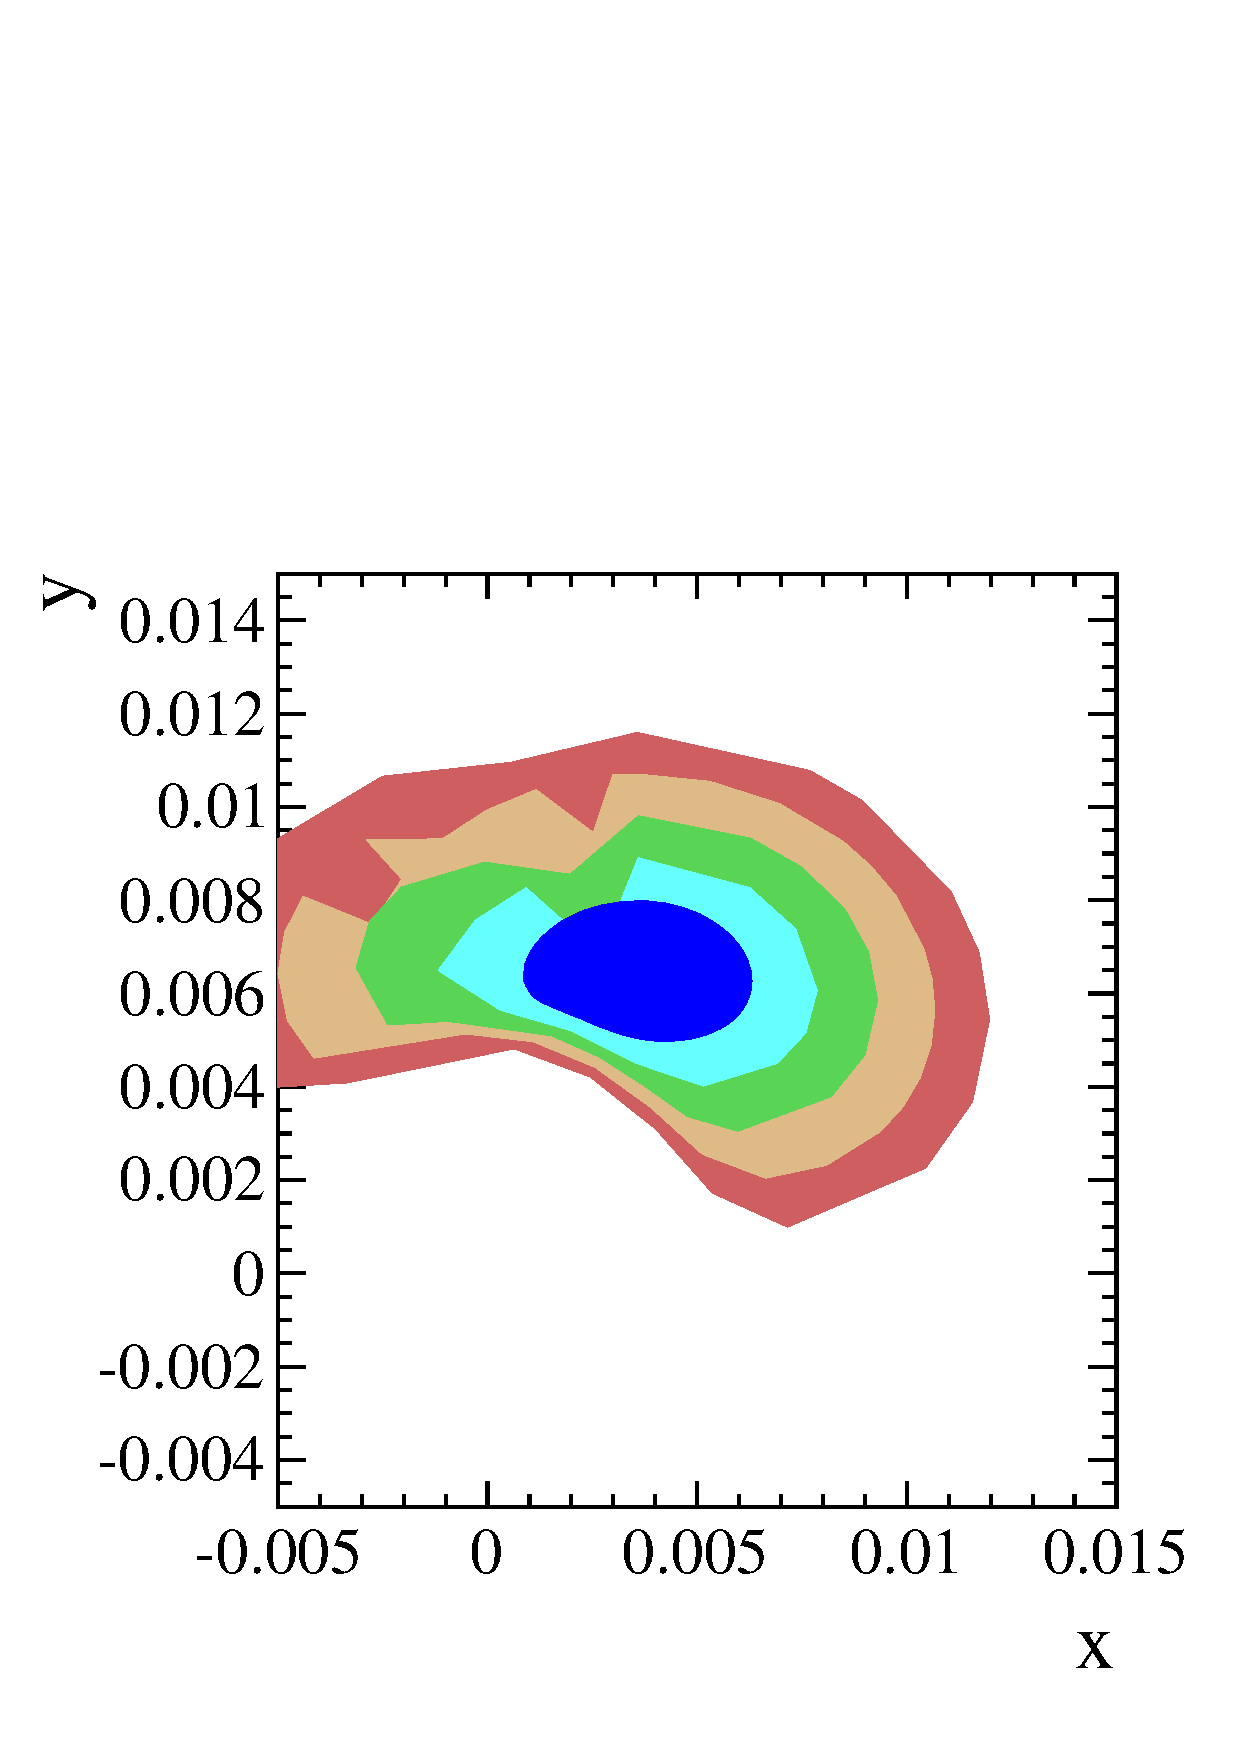
\includegraphics[width=\textwidth]{finalplot_nocpv__graph.pdf}
      \caption{Two dimensional error ellipses for x and y using all available measurements.}
      \label{fig:xy_no_cpv_}
    \end{subfigure}%
    %\hspace{2mm}

    \begin{subfigure}[b]{0.4\textwidth}
      \centering
      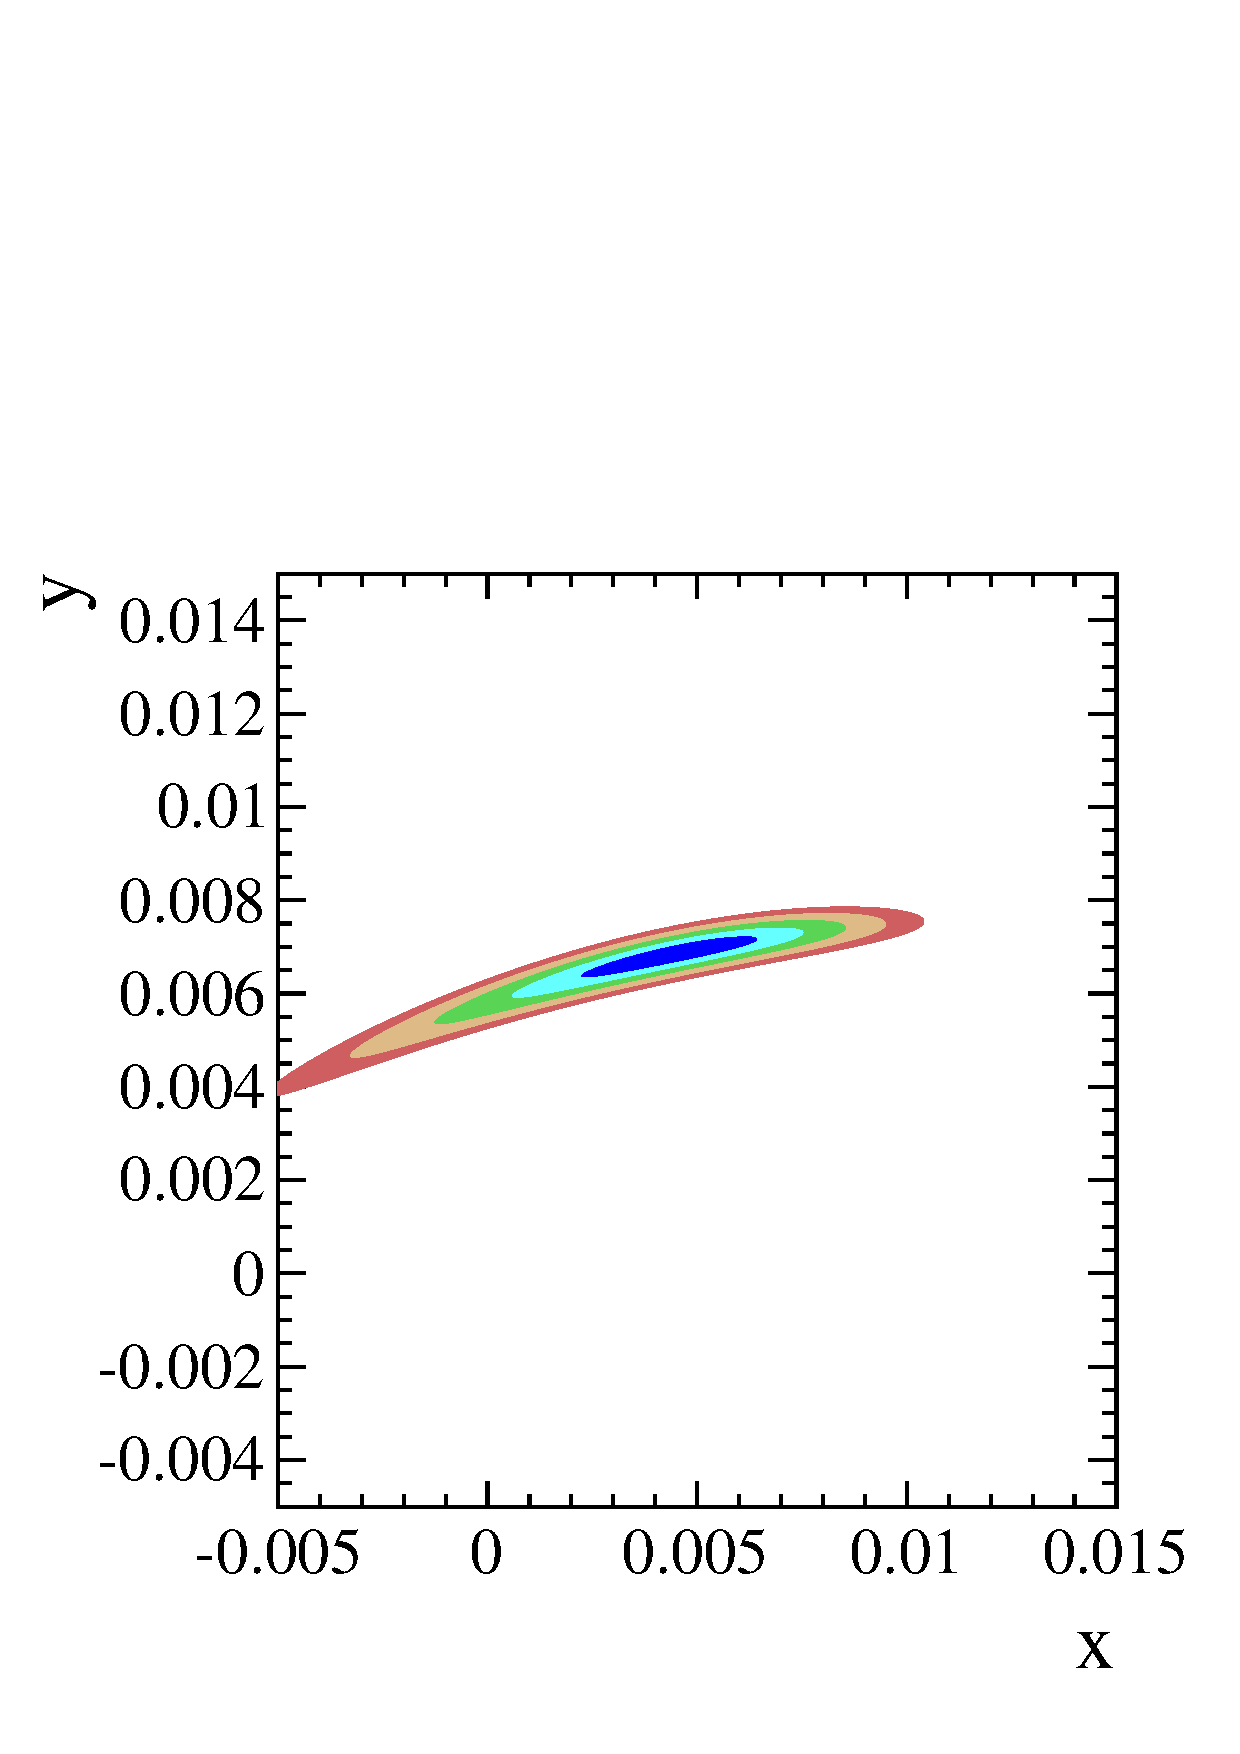
\includegraphics[width=\textwidth]{finalplot_nocpv__belle_babar_graph.pdf}
      \caption{Two dimensional error ellipses for x and y from fit excluding Belle and BaBar $K\pi$ results.}
      \label{fig:xy_no_cpv_nobelle_babar}
    \end{subfigure}%
    \hspace{2mm}
    \begin{subfigure}[b]{0.4\textwidth}
      \centering
      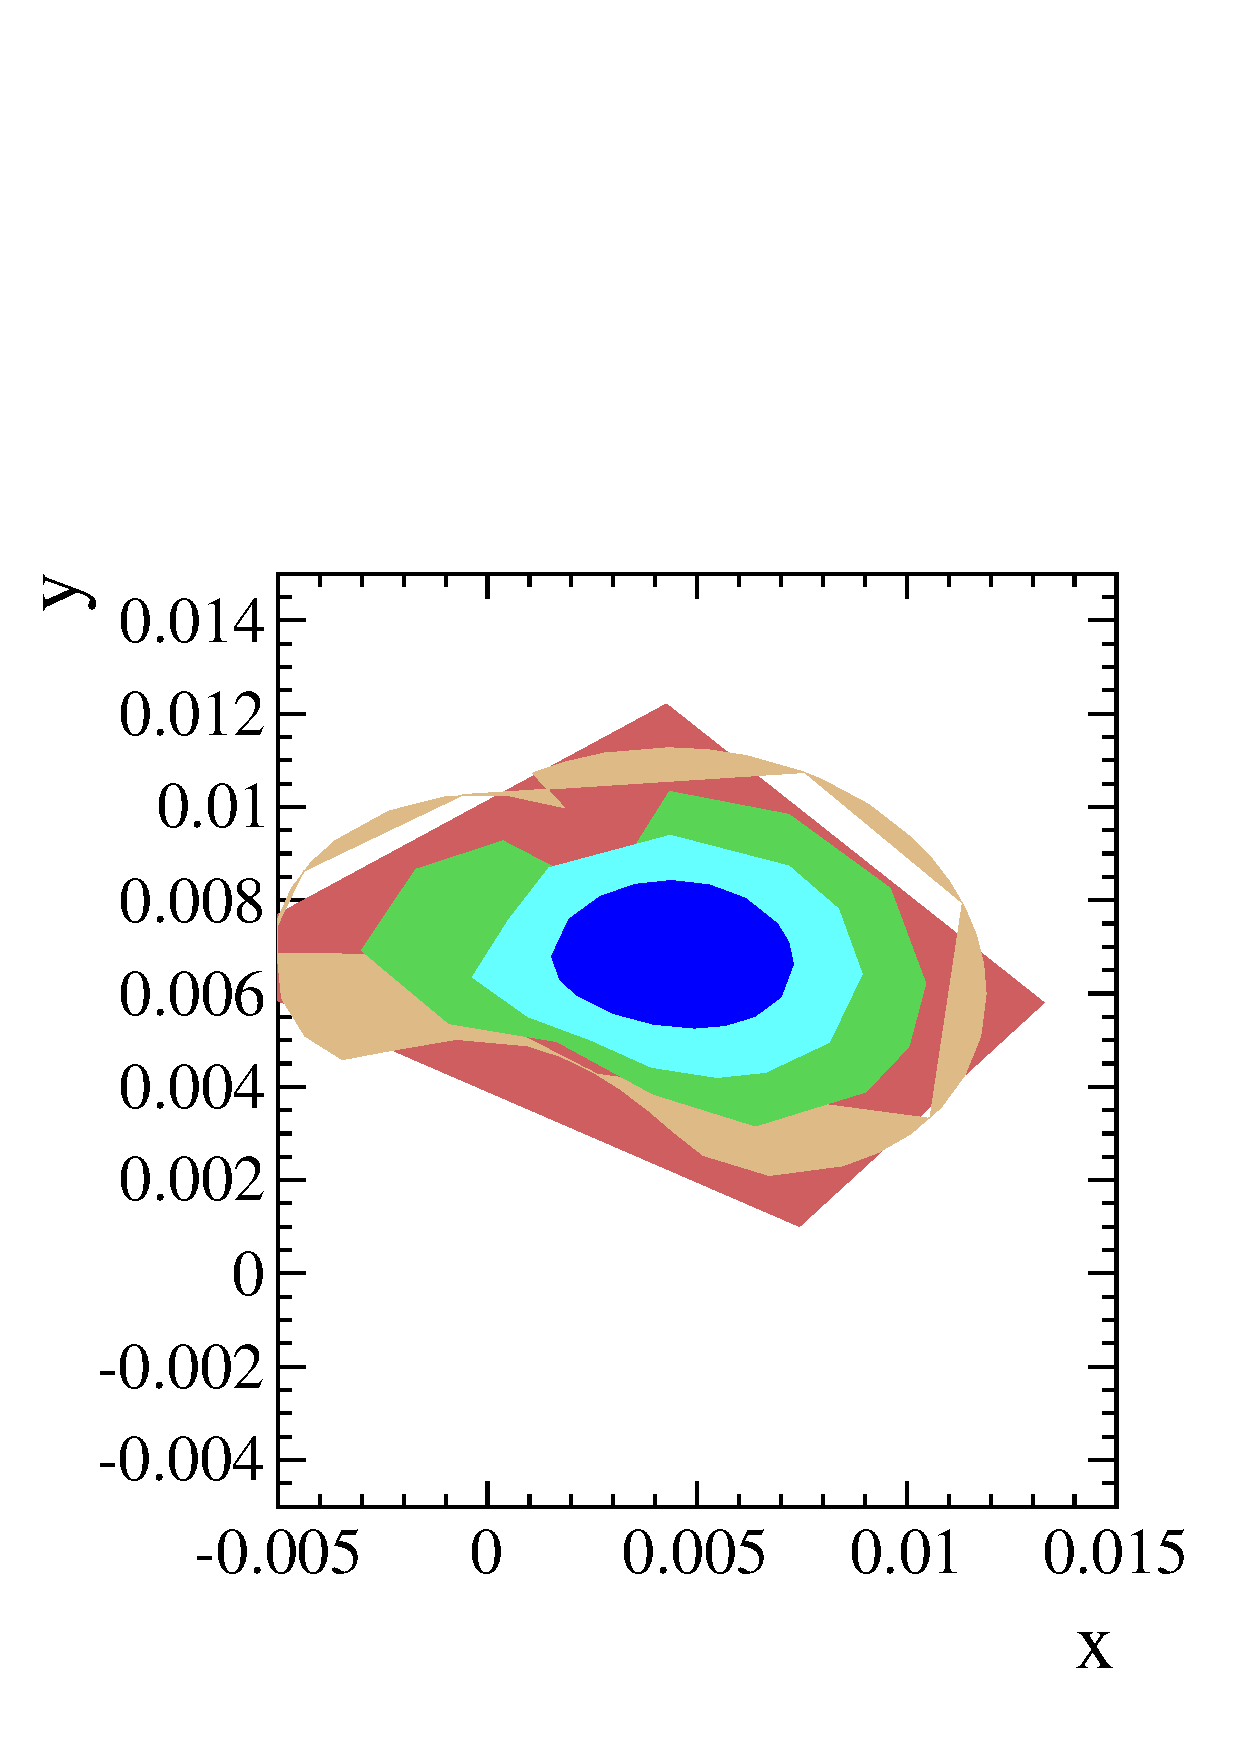
\includegraphics[width=\textwidth]{finalplot_nocpv__belle_babar_cdf_graph.pdf}
      \caption{Two dimensional error ellipses for x and y from fit excluding Belle, BaBar and CDF measurements.}
      \label{fig:xy_no_cpv_nocdf}
    \end{subfigure}%
    %\vspace*{-1.0cm}
  \end{center}
  \caption{Two dimensional error ellipses of $x$ and $y$ from fit for No CPV. Exclusion of the Belle and BaBar results drastically change the slope of the error ellipses. The differing colors represent the 1-5$\sigma$ contours.}
  \label{fig:xy_nocpv_variations}
\end{figure}
\subsection{No Direct CP Violation Allowed}
Table~\ref{table:nodcpv_output_table} lists the results of the global fit of no direct
CP violation. The final three columns of the table represent the effect of the 
inclusion of the preliminary LHCb $A_\Gamma$ result in the global fit.
The inlcusion of this result does not change the central values or errors substantially.

\begin{table}[htdp]
%\begin{tiny}

\begin{center}
\resizebox{16cm}{!} {
\begin{tabular}{|c||c||c||c||c|}
\hline
& All Measurements & No Belle, BaBar$K\pi$& No Belle, BaBar$K\pi$, add $A_{\Gamma\text{ LHCb}}$ & No Belle, BaBar, CDF $K\pi$, add $A_{\Gamma\text{ LHCb}}$ \\ \hline

$x(\times10^{-3})$ & $ 5.191\pm 1.746 $& $4.843\pm 1.782$& $4.845\pm1.782$& $4.844\pm1.787$ \\ \hline

$y(\times10^{-3})$ &$ 6.343\pm 0.905$ & $6.797\pm 1.029$& $6.797\pm 1.030$& $6.809\pm 1.031$ \\ \hline

$\delta_{K\pi}(\times10^{-1})[\text{rad}]$ &$2.468\pm 1.763$ & $3.187\pm 2.021$&$3.188\pm 2.021$ & $3.084\pm 2.040$ \\ \hline

$R_D(\times10^{-3})$ & $ 3.571\pm 0.046 $&$3.555\pm0.046$ & $3.556\pm 0.046$& $3.556\pm 0.047$ \\ \hline

$|q/p|(\times10^{-1})$ & $9.931 \pm 0.125$& $9.935\pm0.135$& $9.929\pm 0.131$ & $9.930\pm0.130 $\\ \hline

$\chi^2/ndf$ & 24.8569/28 & 19.0559/13& 19.3925/15& 8.61793/12\\ \hline

\end{tabular}
}
\end{center}
\caption{Output values of No Direct CPV allowed global fit. Different columns list 
subsets of allowed data.}
\label{table:nodcpv_output_table}
%\end{tiny}
\end{table}%


\subsection{All CP Violation Allowed}
Table~\ref{table:allcpv_output_table} lists the results of the global All CP Violation
allowed fit. Again, the latter columns list the differing subsets of the data to explore
the variation in global $\chi^2/$ndf. The most noticable difference between all fits
is the evaluation of $x$, which varies quite a bit with the inclusion of differing datasets.


%%%%%%%%%%%%%%% XY %%%%%%%%%%%%%%%%%%%%%%%%%
\begin{table}[htdp]
%\begin{tiny}

\begin{center}
\resizebox{16cm}{!} {
\begin{tabular}{|c||c||c||c||c|}
\hline
& All Measurements & No Belle, BaBar& No Belle, BaBar, $A_{\Gamma\text{ LHCb}}$ & No Belle, BaBar, CDF,$A_{\Gamma\text{ LHCb}}$ \\ \hline

$x(\times10^{-3})$& $3.737\pm 1.630$ &$4.817\pm1.688$ &$4.772\pm1.685$ &$4.601\pm1.664$ \\ \hline

$y(\times10^{-3})$& $6.128 \pm 0.743$ & $6.868\pm 0.984$&$6.908\pm0.963$ & $6.956\pm0.867$\\ \hline

$\delta_{K\pi}(\times10^{-1})[\text{rad}]$& $ 1.146\pm 2.127$ & $3.246\pm1.935$& $3.329\pm1.891$& $3.250\pm1.756$\\ \hline

$\phi(\times10^{-1})[\text{rad}]$& $-0.642\pm1.255 $ &$-0.623\pm 1.055$&$-0.651\pm1.046$ & $-1.534\pm1.712$\\ \hline

$R_D^-(\times10^{-3})$& $3.501 \pm 0.040$&$3.568\pm 0.049$& $3.567\pm0.049$&$3.582\pm0.055$ \\ \hline

$R_D^+(\times10^{-3})$& $3.496\pm 0.036$ & $3.547\pm 0.044$ & $3.548\pm 0.043$&$3.533\pm0.046$ \\ \hline

$|q/p|(\times10^{-1})$& $9.631\pm 0.693$& $9.513\pm0.823$&$9.474\pm0.800$ & $8.880\pm1.082$\\ \hline

$\chi^2/ndf$& 59.9402/29 &18.8317/11 & 19.1817/14 & 7.72181/9\\ \hline

\end{tabular}
}
\end{center}
\caption{Output of the All CP Violation allowed global fit. Different Columns list 
differing subsets of data included in the fit.}
\label{table:allcpv_output_table}
%\end{tiny}
\end{table}%

\begin{figure}[htb]
  \begin{center}
    \begin{subfigure}[b]{0.4\textwidth}
      \centering
      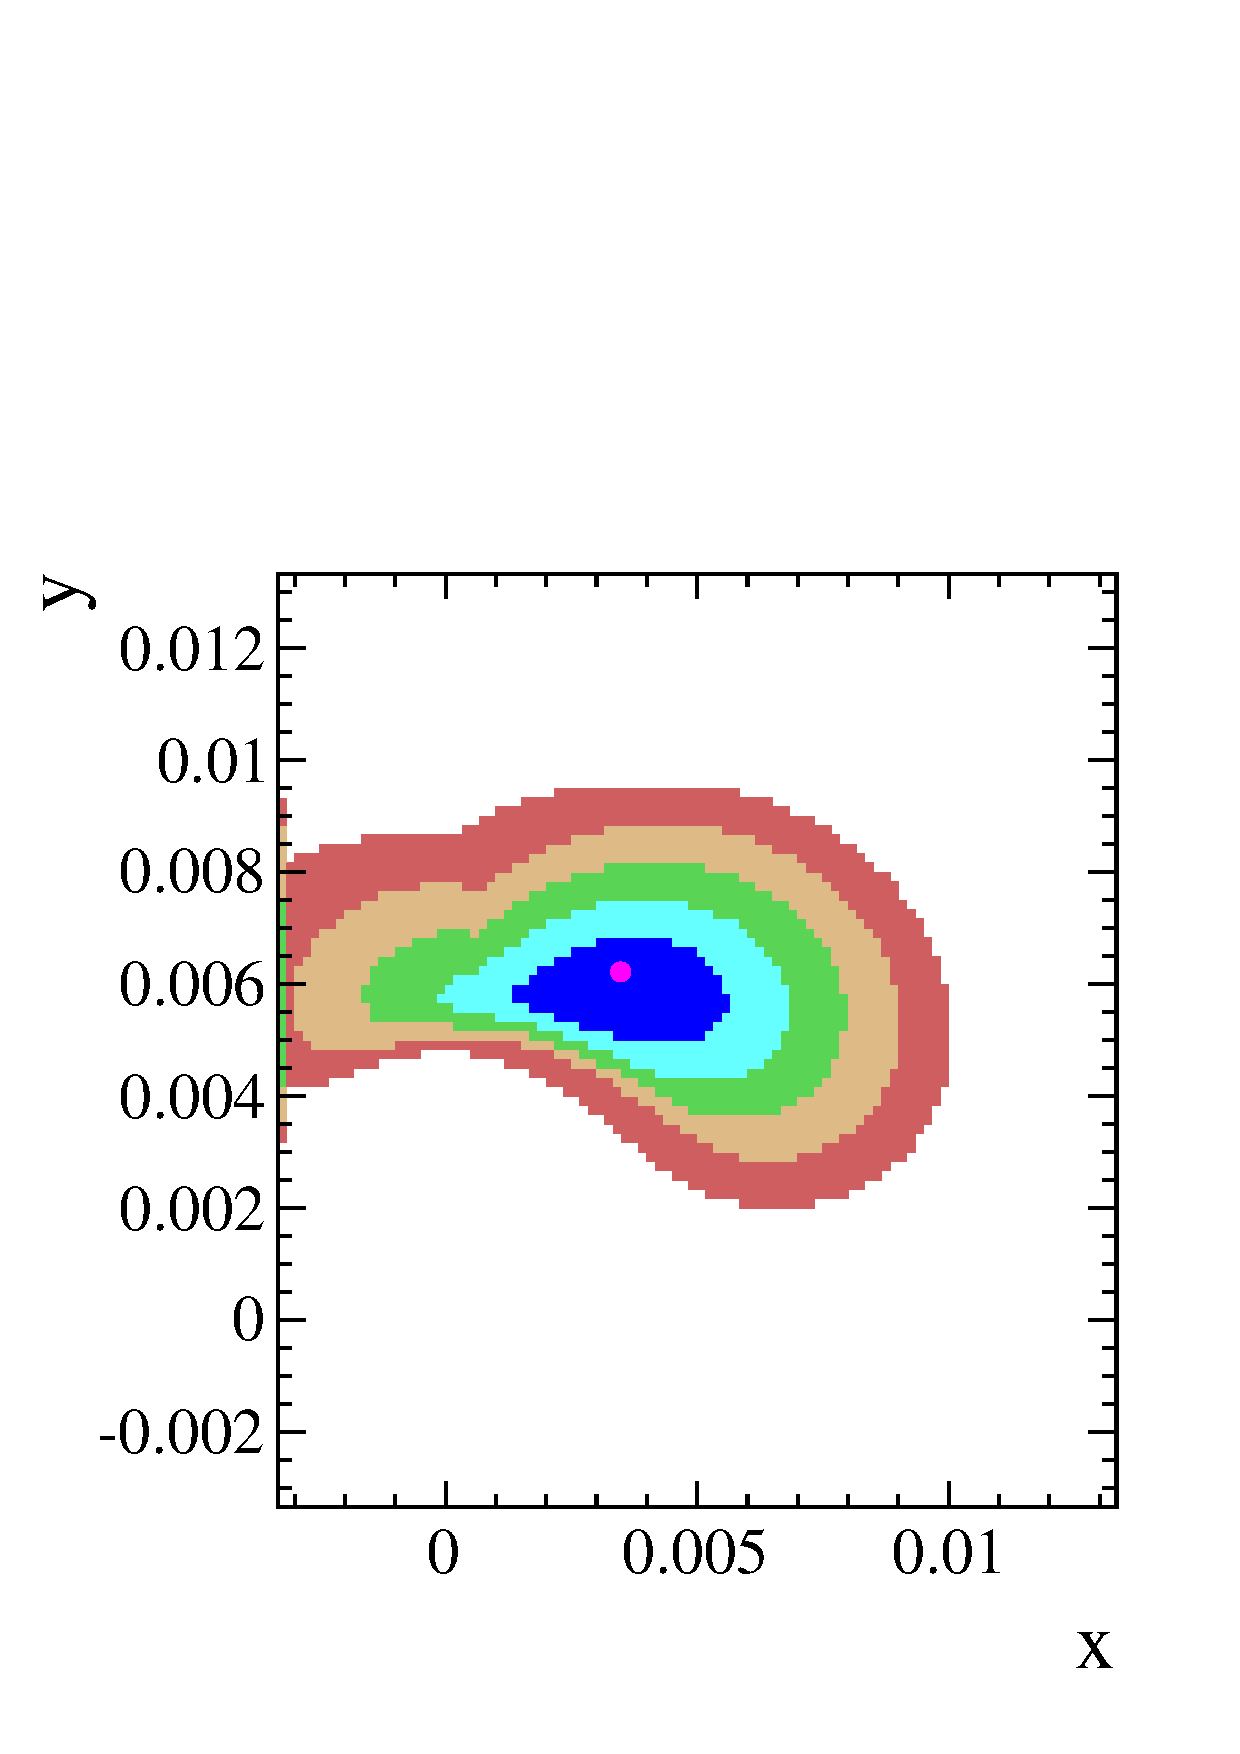
\includegraphics[width=\textwidth]{finalplot_allcpv_no_belle_babar_graph_hfag_agamma.pdf}
      \caption{Two dimensional error ellipses for x and y from fit excluding Belle and BaBar $K\pi$ results. Does not include latest $A_\Gamma$ result of LHCb.}
      \label{fig:xy_all_cpv_no_agamma}
    \end{subfigure}%
    \hspace{2mm}
    \begin{subfigure}[b]{0.4\textwidth}
      \centering
      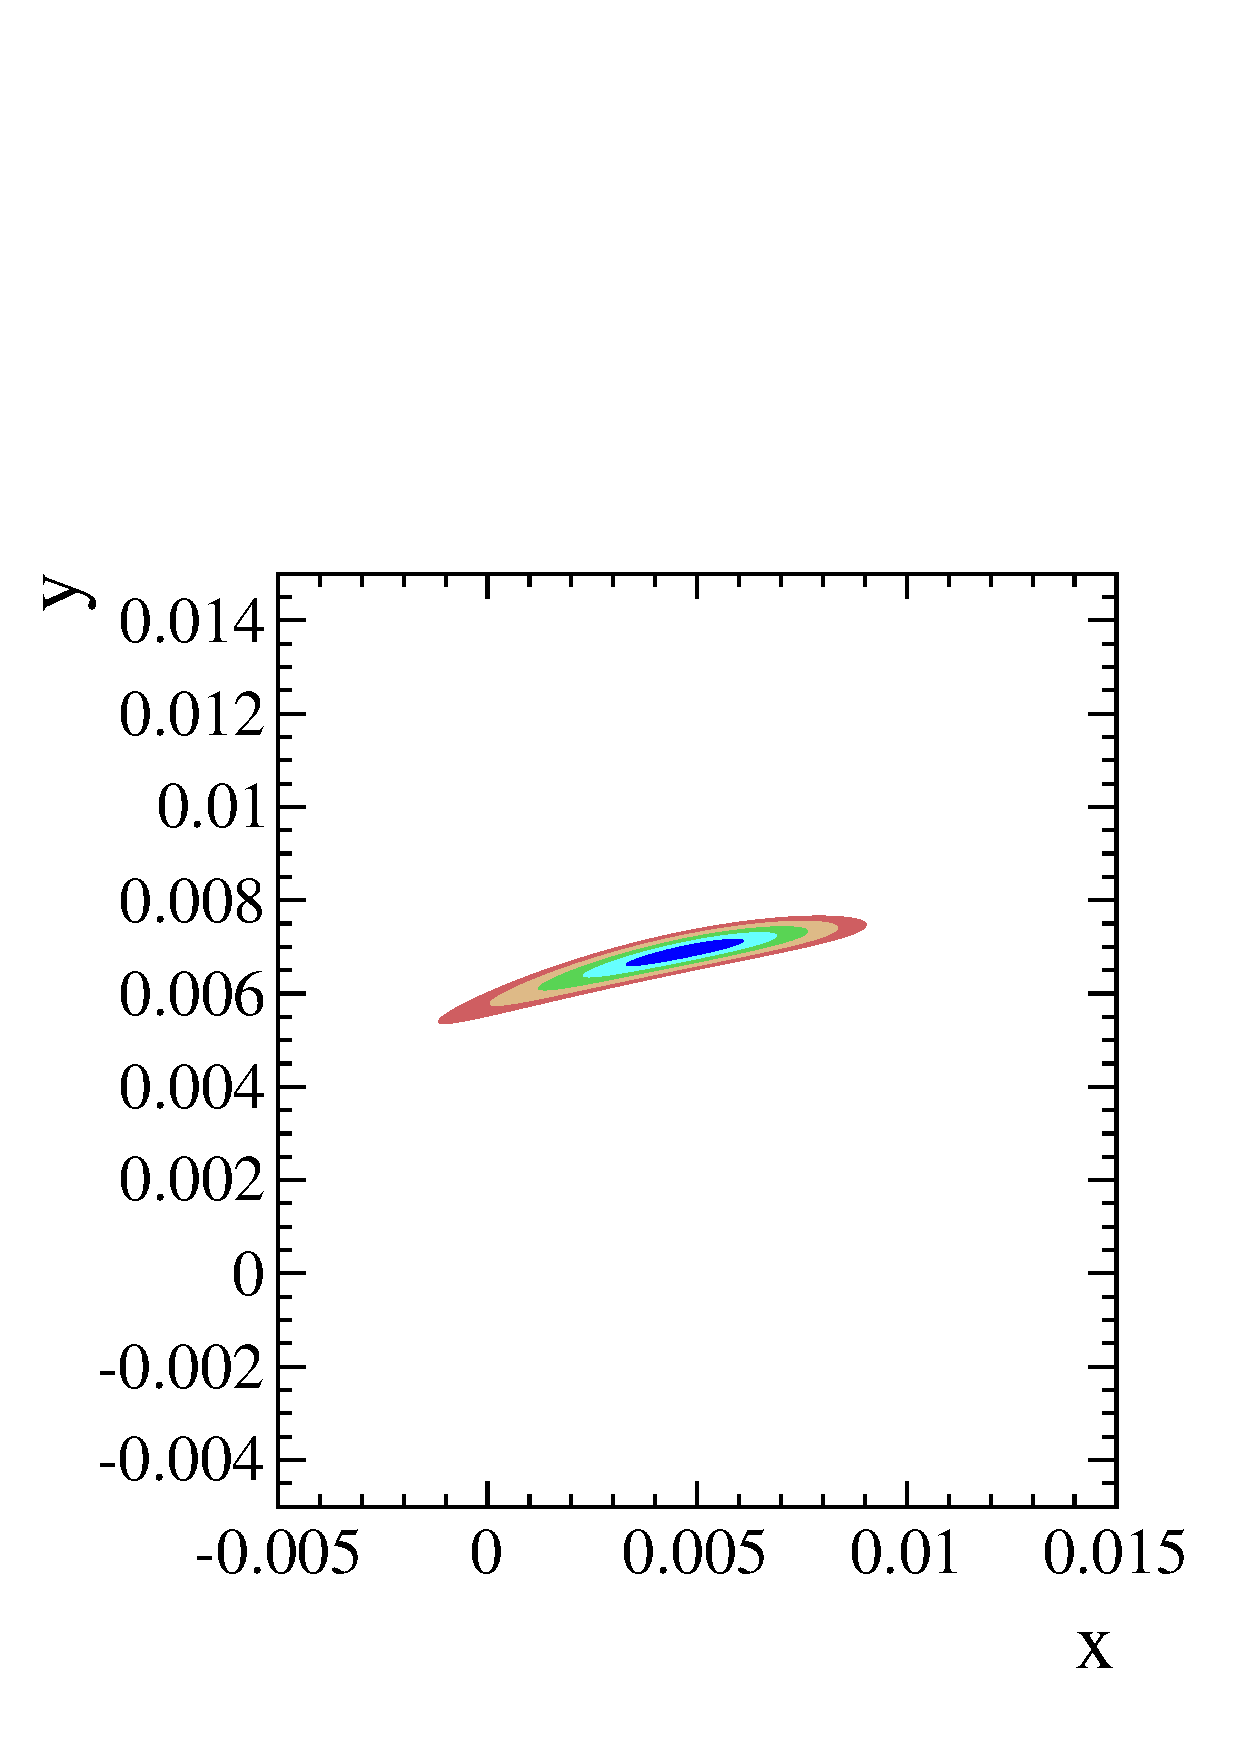
\includegraphics[width=\textwidth]{finalplot_allcpv_no_belle_babar_graph_lhcb_agamma.pdf}
      \caption{Two dimensional error ellipses for x and y from fit excluding Belle and BaBar $K\pi$ results. Include latest $A_\Gamma$ result of LHCb.}
      \label{fig:xy_all_cpv_with_agamma}
    \end{subfigure}%
    \\
%%%%%%%%%
    %\hspace{2mm}
    \begin{subfigure}[b]{0.4\textwidth}
      \centering
      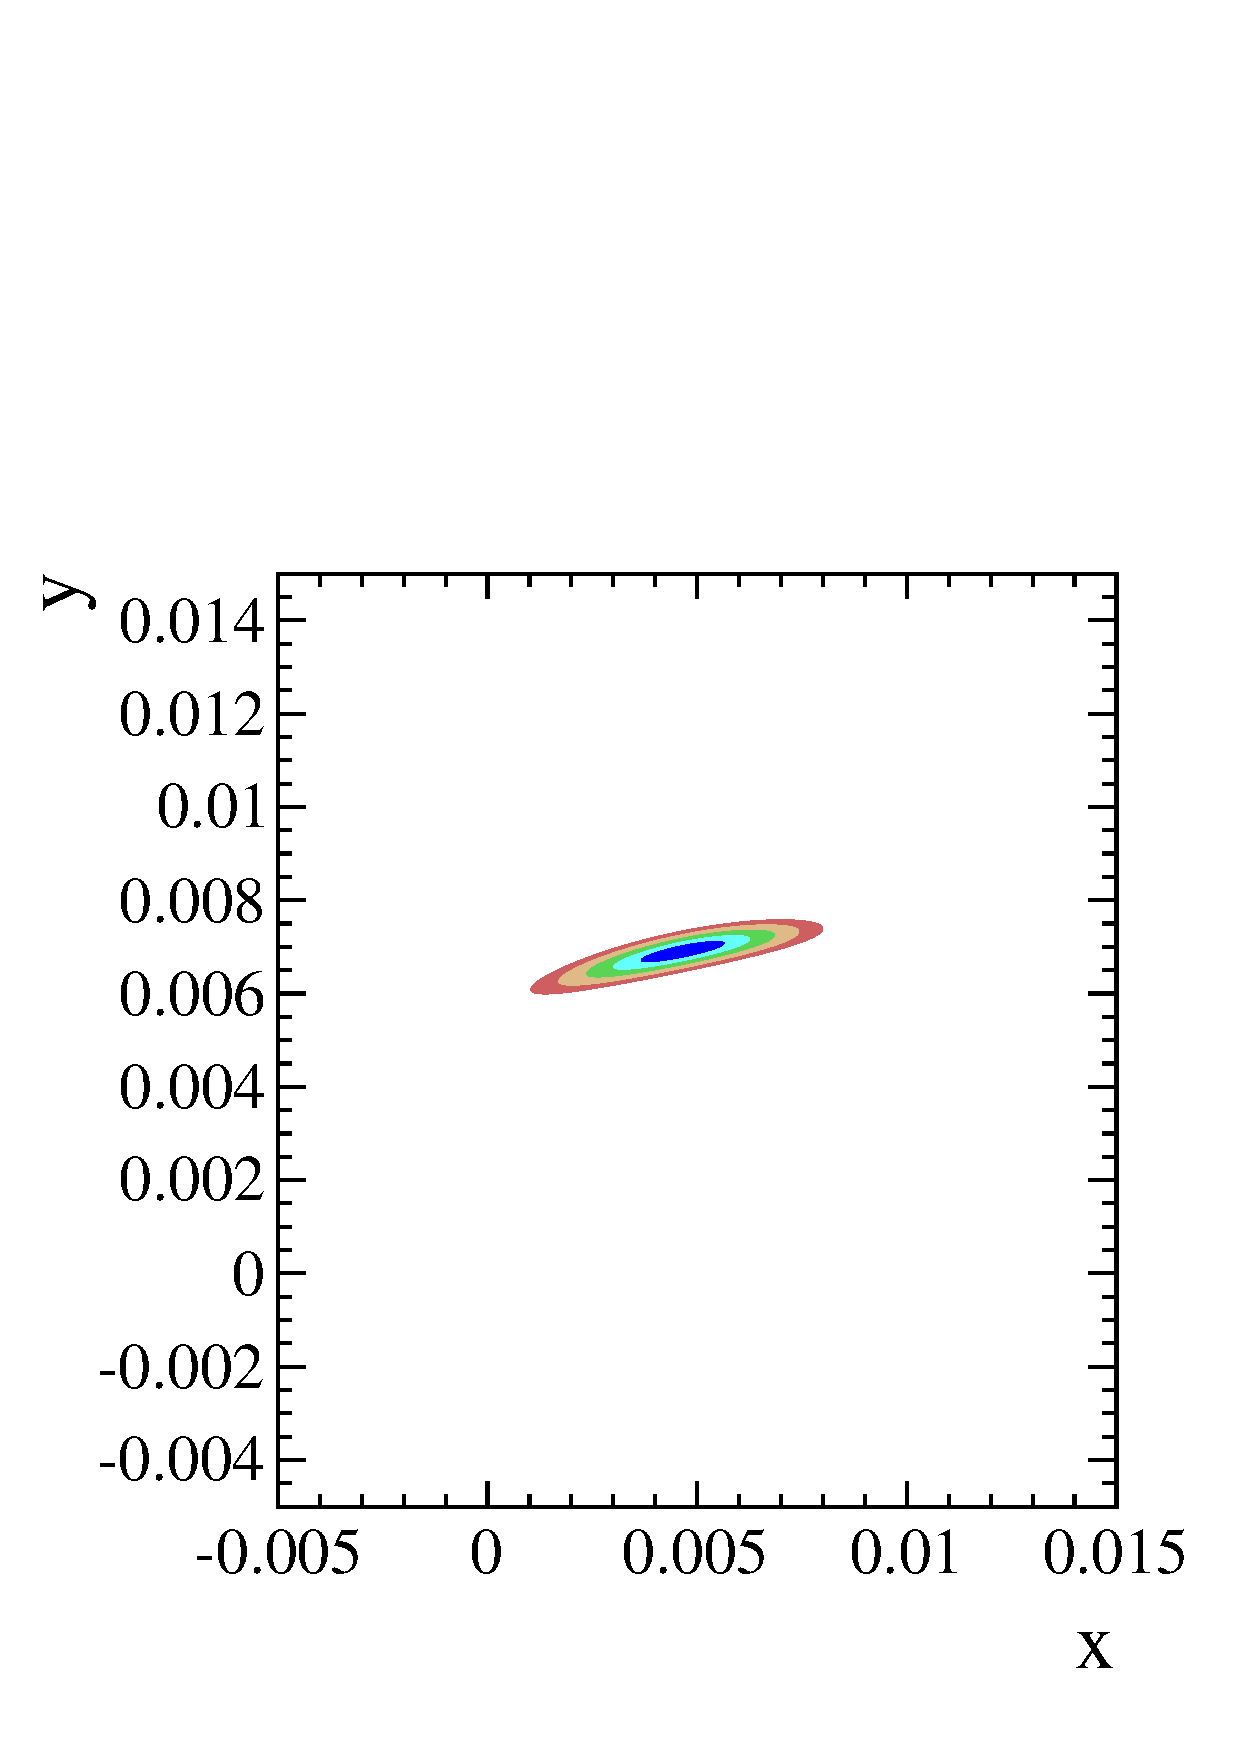
\includegraphics[width=\textwidth]{finalplot_allcpv_no_belle_babar_cdf_graph_hfag_agamma.pdf}
      \caption{Two dimensional error ellipses for x and y from fit excluding Belle, BaBar and CDF $K\pi$ results. Does not include latest $A_\Gamma$ result of LHCb.}
      \label{fig:xy_all_cpv_no_agamma}
    \end{subfigure}%
    \hspace{2mm}
    \begin{subfigure}[b]{0.4\textwidth}
      \centering
      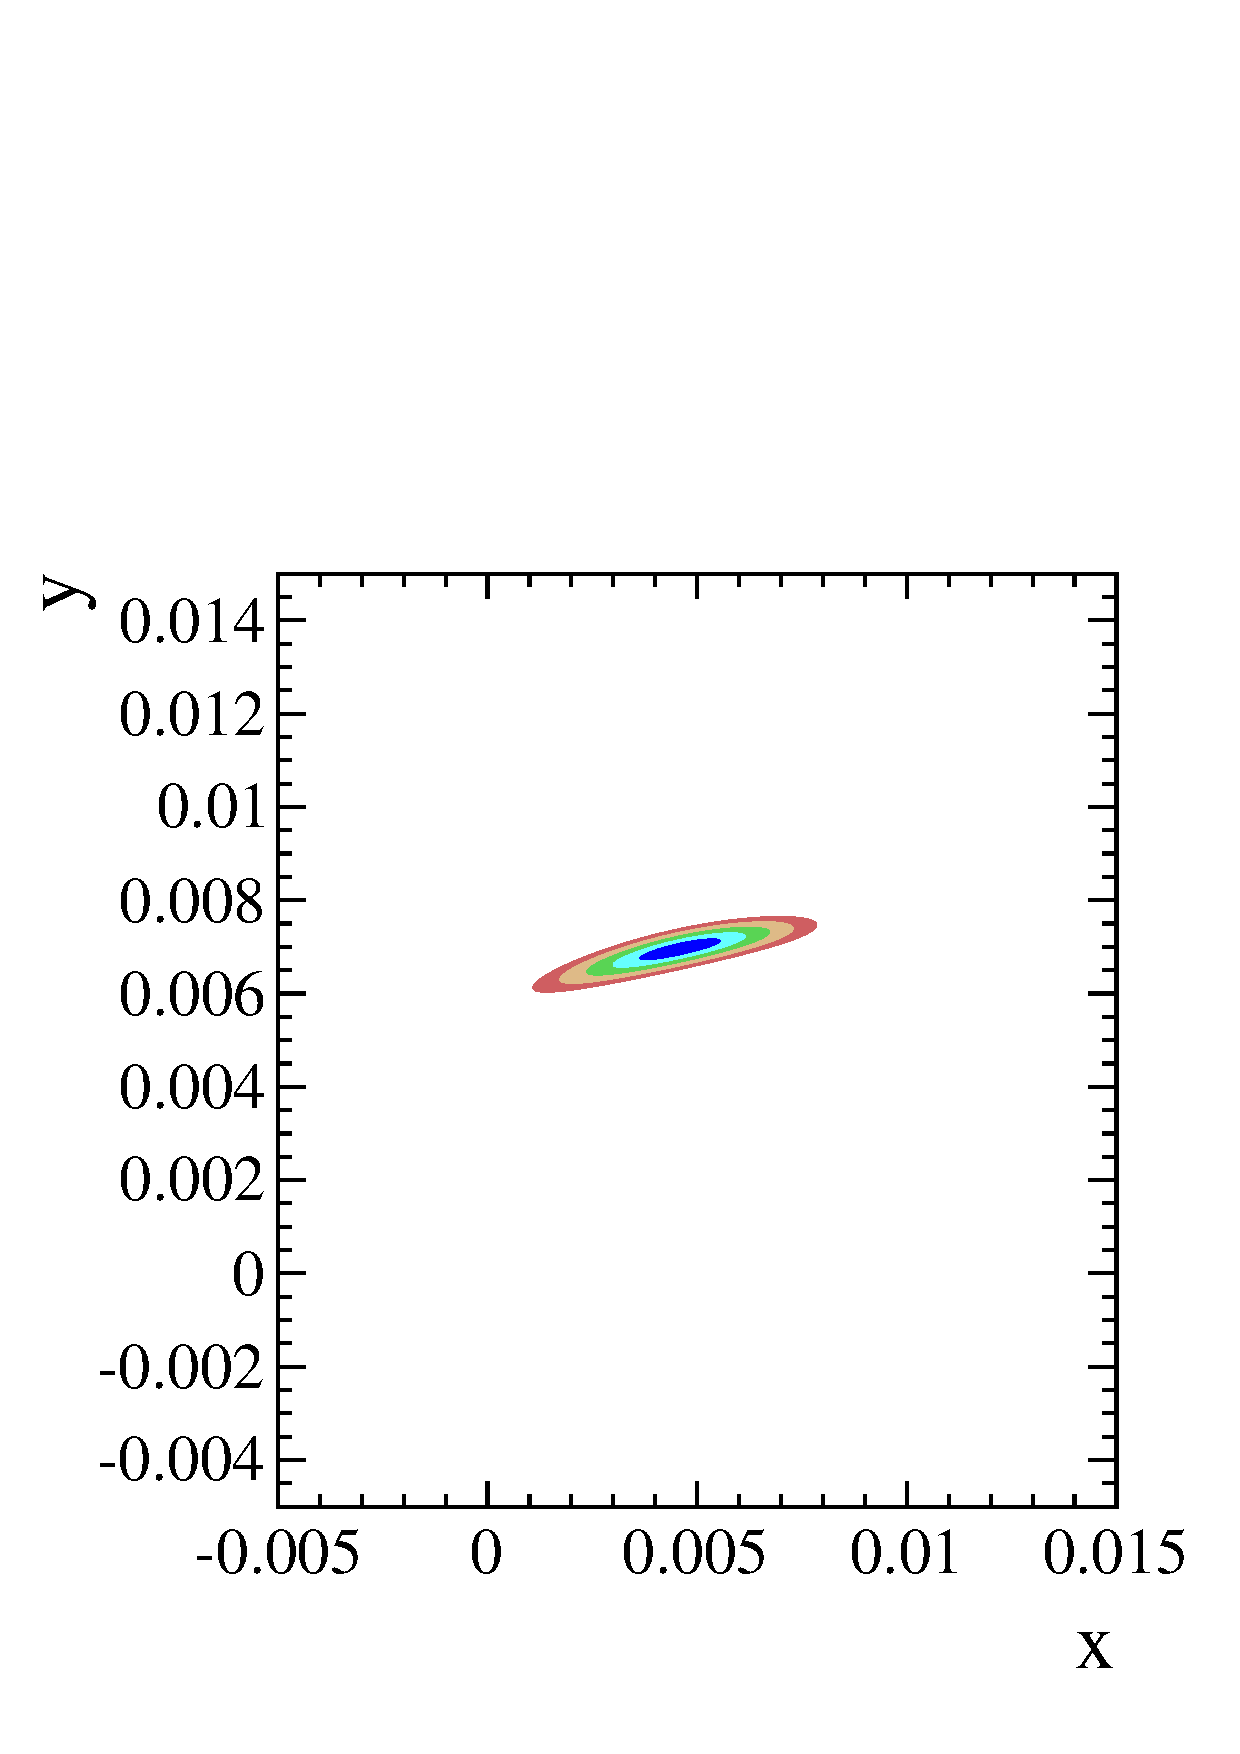
\includegraphics[width=\textwidth]{finalplot_allcpv_no_belle_babar_cdf_graph_lhcb_agamma.pdf}
      \caption{Two dimensional error ellipses for x and y from fit excluding Belle, BaBar and CDF $K\pi$ results. Include latest $A_\Gamma$ result of LHCb.}
      \label{fig:xy_all_cpv_with_agamma}
    \end{subfigure}%
    %\vspace*{-1.0cm}
  \end{center}
  \caption{Two dimensional error ellipses of fit for All CPV including differing sets of data for $x$ vs $y$. The biggest differences come from including the CDF result, which elongates the error ellipses. The differing colors represent the 1-5$\sigma$ contours.}
  \label{fig:xy_all_variations}
\end{figure}

%%%%%%%%%%%%%%%% Q/P %%%%%%%%%%%%%%%%%%%%%%%%%%%%%%%%%%%%
\begin{figure}[tb]
  \begin{center}
    \begin{subfigure}[b]{0.4\textwidth}
      \centering
      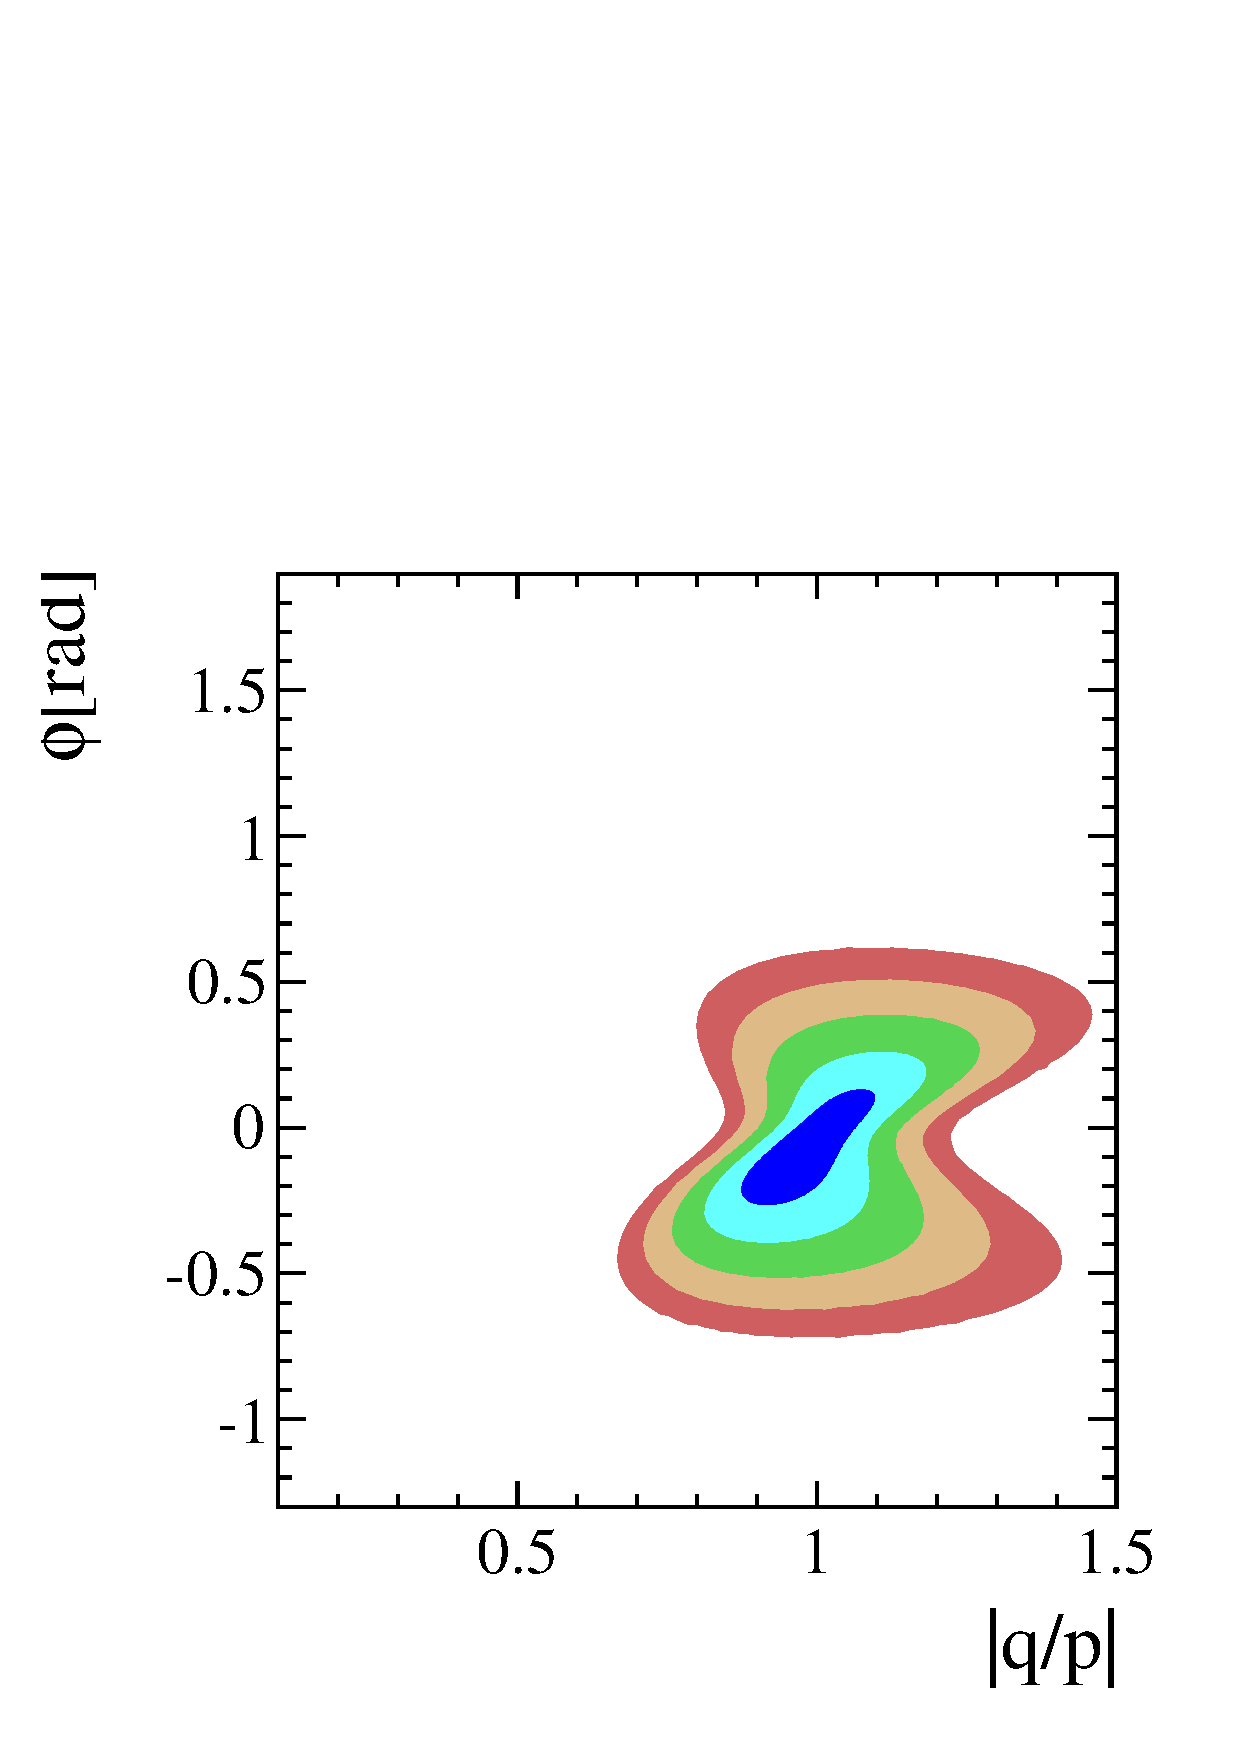
\includegraphics[width=\textwidth]{finalplot_allcpv_no_belle_babar_graph_qop_phi_hfag_agamma.pdf}
      \caption{Two dimensional error ellipses for x and y from fit excluding Belle and BaBar $K\pi$ results. Does not include latest $A_\Gamma$ result of LHCb.}
      \label{fig:xy_all_cpv_no_agamma}
    \end{subfigure}% 
    \hspace{2mm}
    \begin{subfigure}[b]{0.4\textwidth}
      \centering
      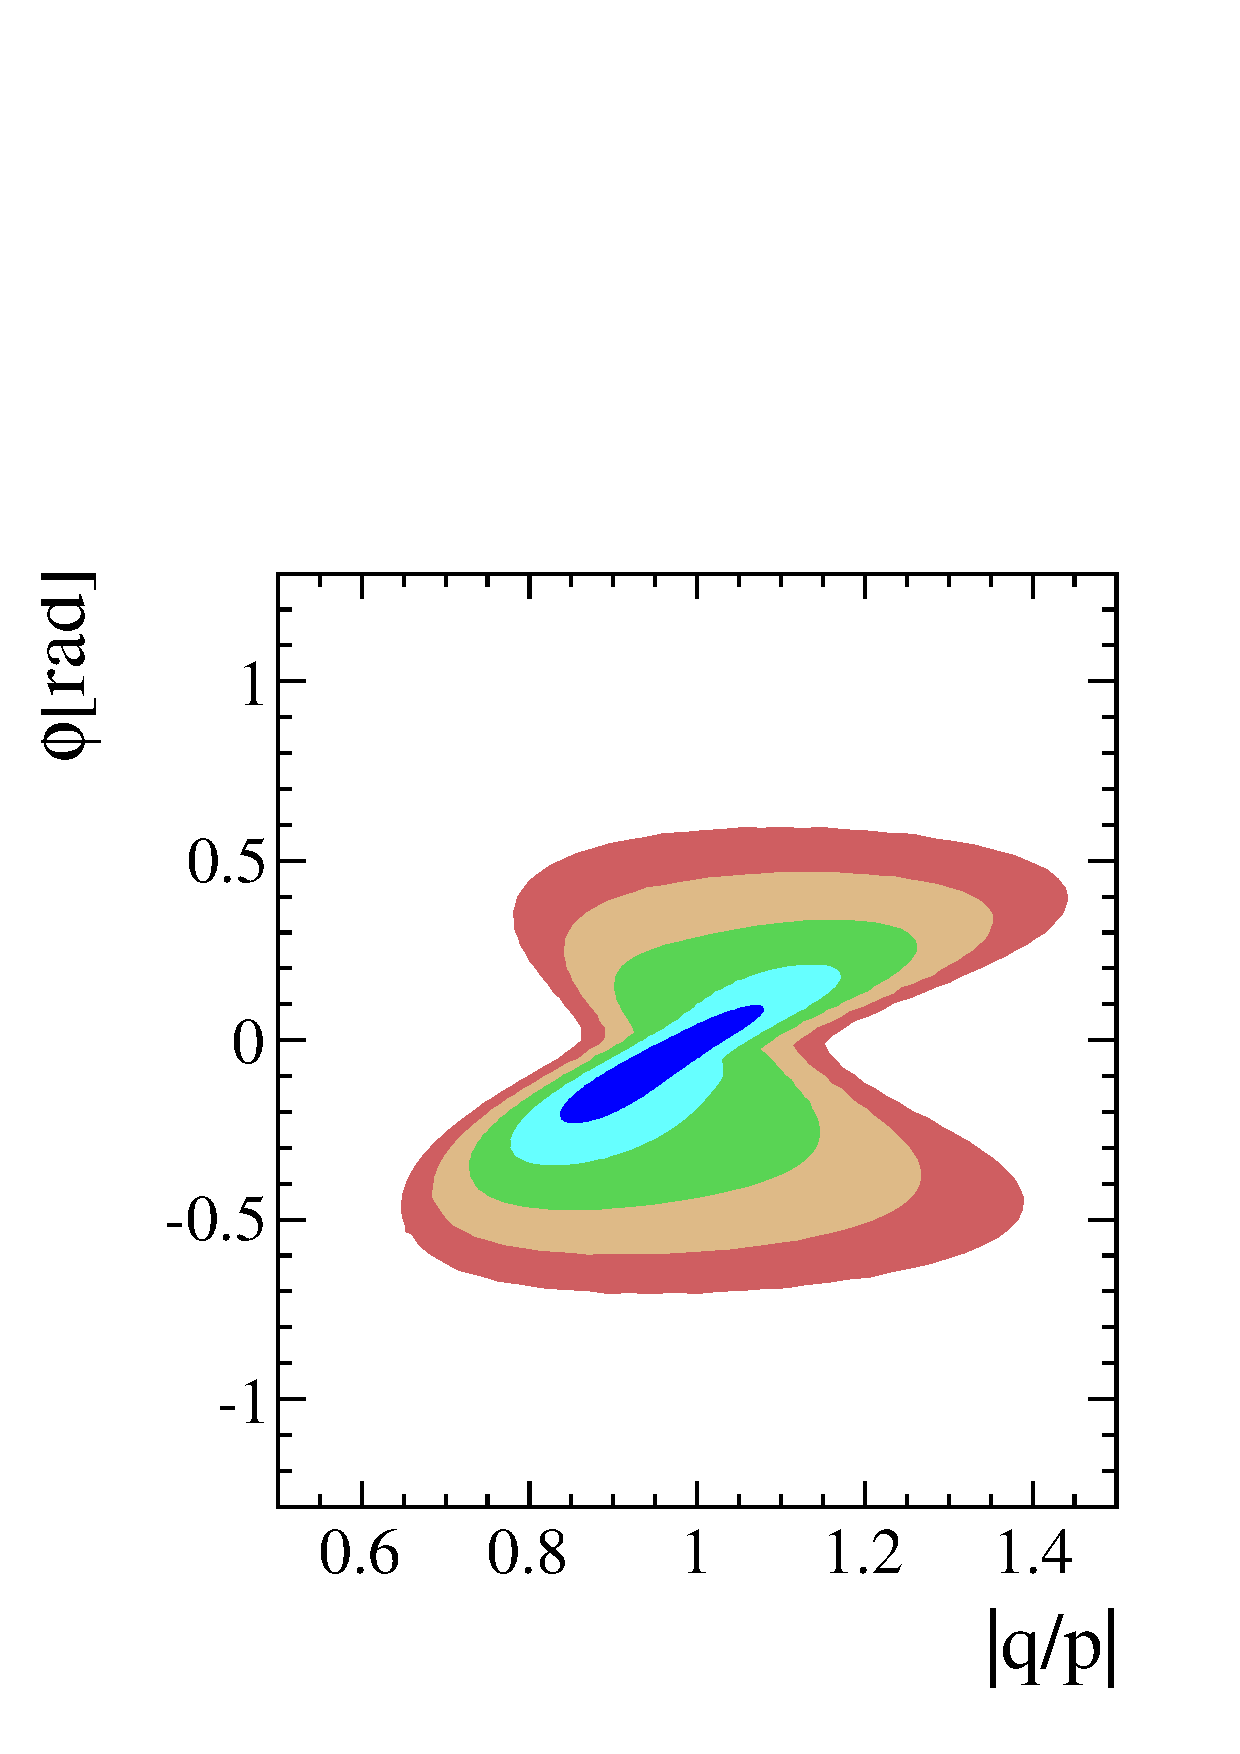
\includegraphics[width=\textwidth]{finalplot_allcpv_no_belle_babar_graph_qop_phi_lhcb_agamma.pdf}
      \caption{Two dimensional error ellipses for x and y from fit excluding Belle and BaBar $K\pi$ results. Include latest $A_\Gamma$ result of LHCb.}
      \label{fig:xy_all_cpv_with_agamma}
    \end{subfigure}%
%%%%%%%%%
        \\
    \begin{subfigure}[b]{0.4\textwidth}
      \centering
      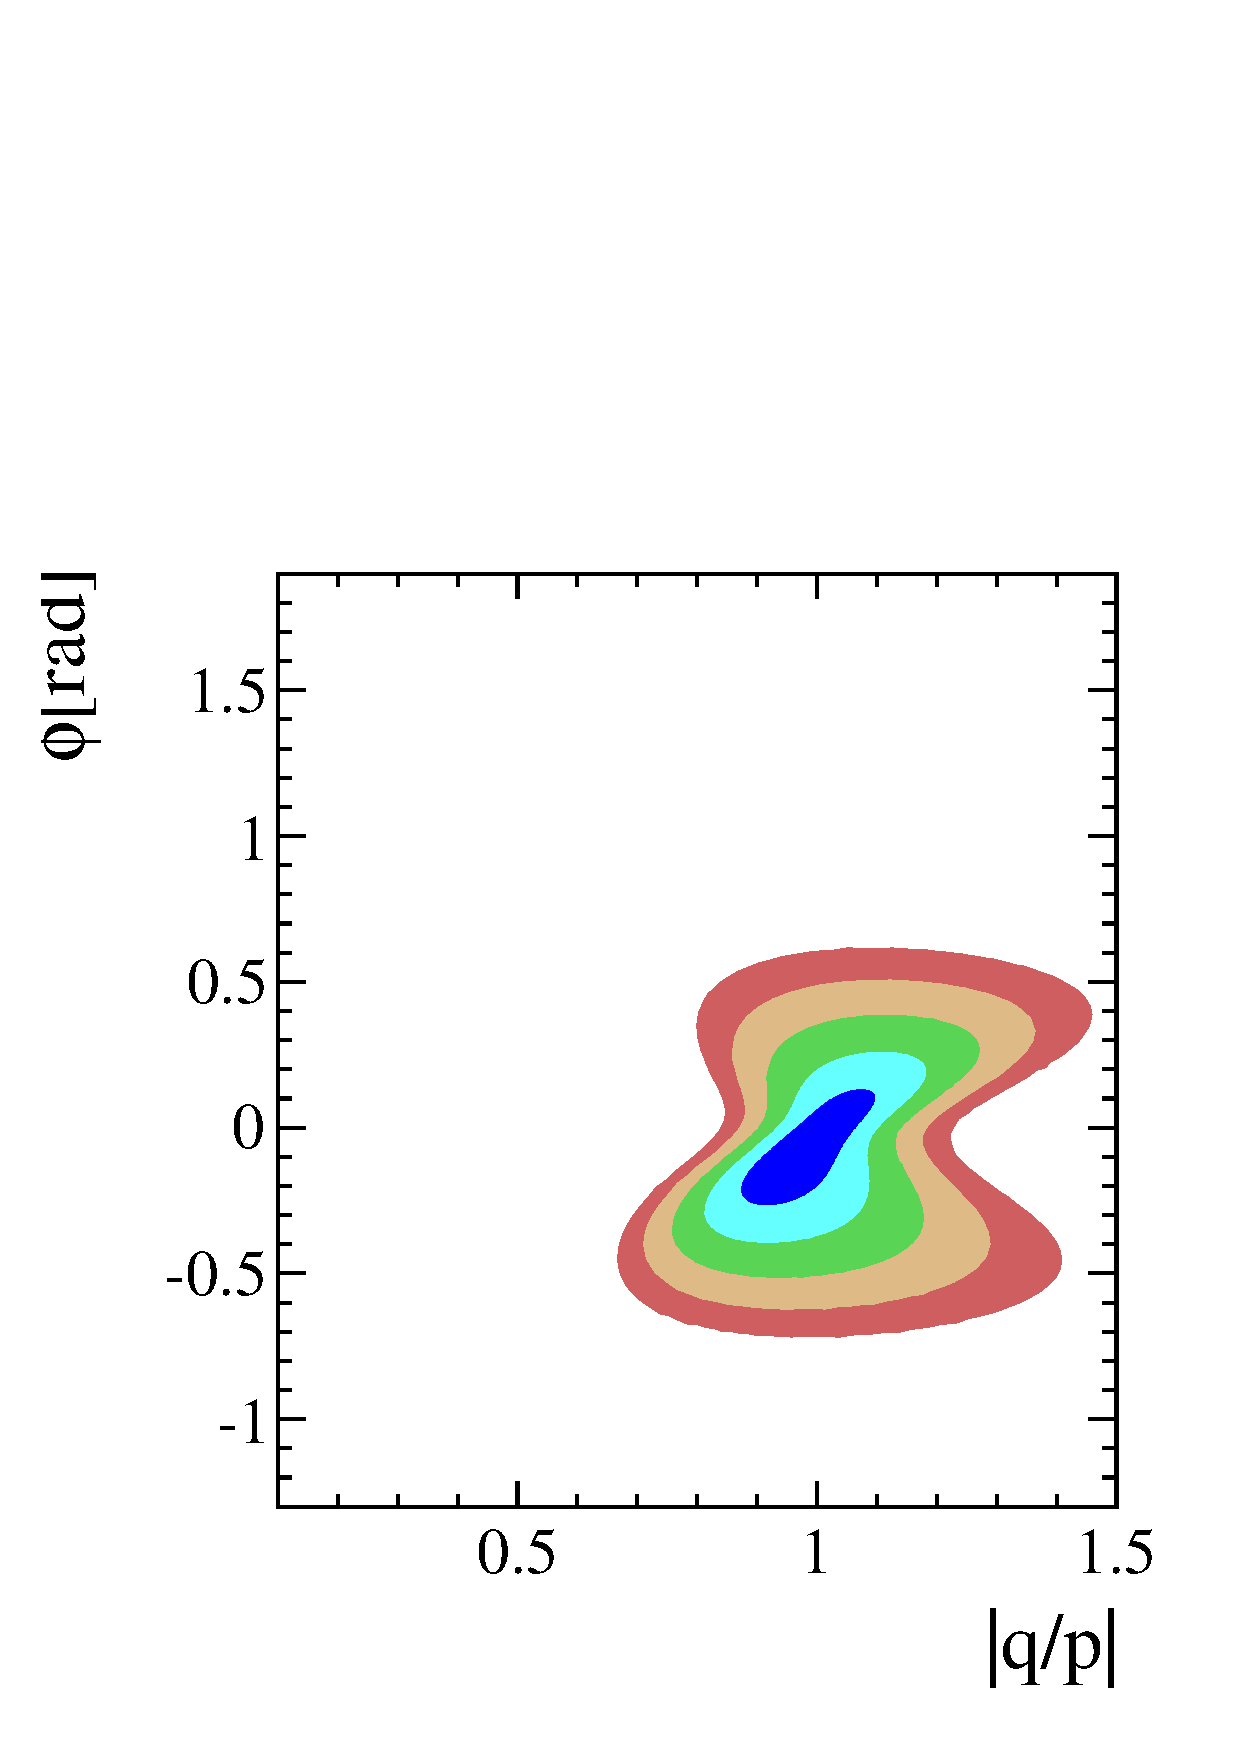
\includegraphics[width=\textwidth]{finalplot_allcpv_no_belle_babar_cdf_graph_qop_phi_hfag_agamma.pdf}
      \caption{Two dimensional error ellipses for x and y from fit excluding Belle, BaBar and CDF $K\pi$ results. Does not include latest $A_\Gamma$ result of LHCb.}
      \label{fig:xy_all_cpv_no_agamma}
    \end{subfigure}%
    \hspace{2mm}
    \begin{subfigure}[b]{0.4\textwidth}
      \centering
      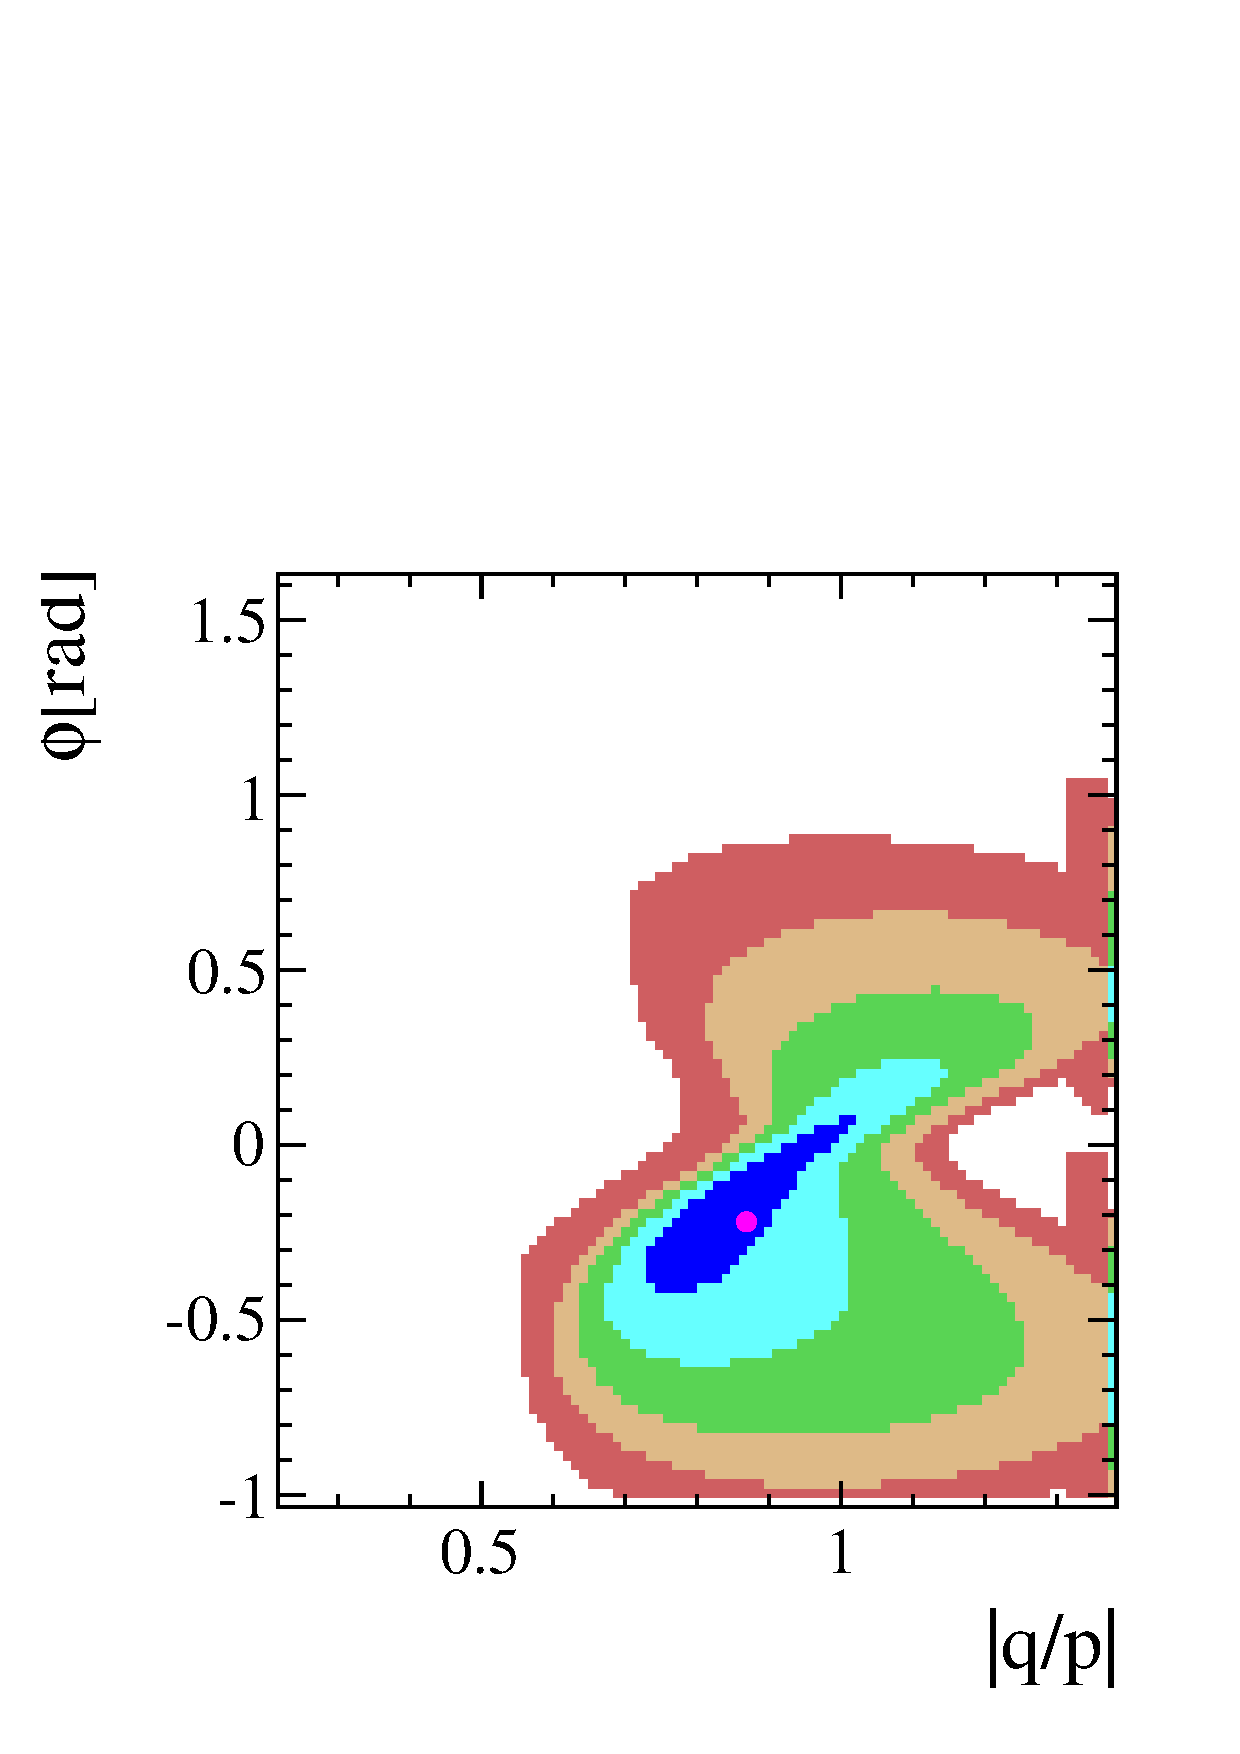
\includegraphics[width=\textwidth]{finalplot_allcpv_no_belle_babar_cdf_graph_qop_phi_lhcb_agamma.pdf}
      \caption{Two dimensional error ellipses for x and y from fit excluding Belle, BaBar and CDF $K\pi$ results. Include latest $A_\Gamma$ result of LHCb.}
      \label{fig:xy_all_cpv_with_agamma}
    \end{subfigure}%
    %\vspace*{-1.0cm}
  \end{center}
  \caption{Two dimensional error ellipses of fit for All CPV including differing sets of data for $\phi$ vs $q/p$. The biggest differences come from including the CDF result, which elongates the error ellipses. The differing colors represent the 1-5$\sigma$ contours.}
  \label{fig:xy_all_variations}
\end{figure}
